\chapter{Discussion and Future Work}
\textit{FlexTouch} enables large-scale interaction sensing beyond the spatial constraints of capacitive touchscreens by introducing the local ground into the extension circuit design. We show that our technique is compatible with a variety of conductive materials as well as fabrication methods. \textit{FlexTouch} supports posture recognition, human-object interaction as well as enhanced fitness training experiences with a large coverage range of up to 4 meters. In this section, we discuss our findings, design guidelines, and future work. 
\section{Lower Development Barriers Using \textit{FlexTouch}}
Since \textit{FlexTouch} requires no external or internal hardware modifications, our technique allows end-users to design and develop varied, low-cost capacitive sensing applications easily with a single touchscreen device. In addition, they can fabricate the customized low-cost interface with various commercially available materials and fabrication methods. 

\section{Effectiveness and Limitation of Introducing the Local Ground to Boost the Sensing Range}
\textit{FlexTouch} enables long-range capacitive sensing of up to 4 meters by introducing the local ground of the touchscreen to the extension circuit design. Through a series of studies, we proved the effectiveness of this approach. In addition, we found some insightful results that may benefit future designs. We recommend thinner, more conductive material to make extension strips and wider gap distances between grounding and signal strips to achieve a better sensing performance.

However, the limitation of this "local ground" method is the low spatial resolution and the effort to avoid overlays between the signal and grounding strips. Designers can choose to increase the resolution by shortening the gap distance and reducing the sensing range. We recommend a multi-layer design to avoid the intersection between signal and grounding strips as Section $6.1$ and $6.2$ shows. One potential solution to this limitation is connecting users or objects to the local ground directly with conductive threads. Another possible solution is connecting the local ground to the earth ground through a charging line. Therefore, the environmental virtual ground couples the human body and earth ground to the local ground of touchscreen devices. 

\section{Fabrication and Assembly}
We demonstrated that \textit{FlexTouch} is compatible with four commercially available fabrication materials as well as a variety of fabrication methods. The current fabrication of our system is primarily based on hand-made prototypes. Additional machine-based approaches are expected for volume production with better quality control. We propose several potential directions for fabrication such as conductive inkjet printing, laser cutting with conductive frames, or printing robots that can enable large-scale circuit design on a wall \footnote{https://scribit.design/}. Programmable sewing machines can extend FlexTouch applications to touch interface widgets on a sleeve for quick access to a phone placed in a pocket.

In addition to our existing plug and play approaches in Section $4.3$, we expect additional approaches to further extend this idea. For instance, future design can enable an electrode base where users can lay their phone with the touchscreen facing downward to connect to \textit{FlexTouch} interfaces. Furthermore, since the conductive strip increases the raw capacitive value when it's attached to the touchscreen, we can connect different applications with a patterned strip array. \textit{FlexTouch} can detect the signal pattern caused by the patterned strip to serve as a short for launching applications when users attach the extension circuit to the touchscreen.

We recommend future fabrication designs considering the layout and spatial resolution when placing sensing nodes. An improper design leads to low recognition accuracy result as section 6.1 (smart mattress) demonstrates. The distance between sensing nodes is approximately 30 cm. As a result, it is hard for this application sensing users' sitting posture when they sit in the gap between electrodes or on the edge of the mattress. We believe that a higher resolution will improve accuracy significantly. In addition, we observed the negative effect of cloths on the signal strength especially with the presence of the sheet. Therefore, future designs should also consider the object/cover placed between human bodies and the extension surface.

\section{The Effect of Resistance of the Extended Material}
We identified four kinds of materials for \textit{FlexTouch} including copper foil tape, ITO PET plastic film, carbon paint and silver nanoparticle ink. The resistance of these materials varies from $0.2 \Omega$ per square centimeter to several kilos $\Omega$ per square centimeter. We did not discuss the effect of the material's resistance in the \textit{Working Principle} section. However, the resistance introduced by the material will have a significant effect on the signal strength once it reaches to kilos $\Omega$ according to prior work ~\cite{mobicom-gao18}. We will explore the feasibility of utilizing both the capacitance and resistance introduced by the extension of conductive 2D patterns in the future. 

\section{Enabling More Sensing Nodes}
Currently, only the sensing nodes on the edge of the touchscreen have been used (94 nodes for the P20 phone and 88 nodes for the P10 phone). In the future, we can extend more nodes with a cover (Fig \ref{fig:3d layout}) that can be attached to the touchscreens. Multiple layers can be attached to different columns of the touchscreen with isolated materials between layers. By activating more sensing nodes, we can increase the resolution and range of our applications, which provide us with more possibilities. Another solution to enable more sensing nodes is designing the extension layout in an X-Y matrix configuration as shown in Section $6.3$. To minimize the effect between neighboring sensing electrodes, we suggest a gap between attached strips larger than $2 mm$ on the touchscreen. We also suggest an isolation gap between layers into which we inserted a $4mm$ isolated rubber in each joint node. 

\begin{figure}[ht]
\centering
  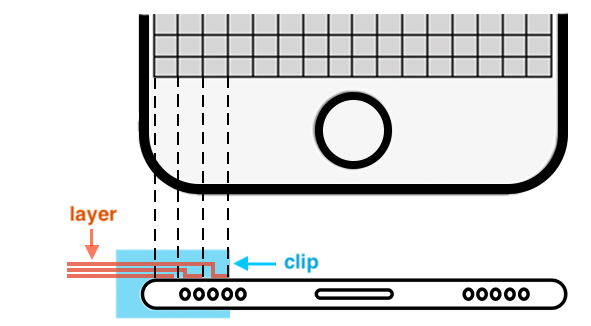
\includegraphics[width=0.25\columnwidth]{figures/3d_layout.png}
  \setlength{\belowcaptionskip}{-6pt}
  \caption{Possible design for more sensing nodes. }
  \label{fig:3d layout}
\end{figure}

\section{Conclusion}
\textit{FlexTouch} enables large-scale, passive, and low-cost interaction sensing interfaces by extending the capacitive sensing capability of touchscreens into the ambient environment. It can support a variety of large-scale interaction applications by attaching customized conductive strips to the edge of the touchscreen. We demonstrated that our technique allows for easy fabrication of touch interfaces via a variety of commercially available conductive materials and fabrication approaches. Through a series of evaluation studies, we showed that \textit{FlexTouch} supports long-range touch interaction sensing for up to 4 meters as well as everyday object presence detection for up to 2 meters. Then we demonstrated the versatility and feasibility of \textit{FlexTouch} by implementing and evaluating applications in the domain of body posture recognition, activity detection, object presence detection, and enhanced fitness tracking experiences.